%\chapter{Different Proof Techniques for demonstrating Turing Completeness}
\chapter{Different Approaches for Proofs to Demonstrate Turing Completeness}

\section{Overview}

We will be exploring the different approaches to demonstrate TC for different systems.
I have oultined the approaches based on their respective discipline.
I hope that this allows for the logic to be legible and digestible.
My intention is to add clarity on where the logic behind these proofs/techniques exist.
For example, in the Computer Engineering perspective, they analyze the TM based on its mechanical properties such as Addition, Logic Gates and so forth.
This is vastly different compared to how Mathematicians show TM and TC, which is through the use of Lambda calculus which is a model for representing functions as a basic unit.
However, all proofs are equivalent in goal.
These are not the only perspectives and types of proofs for showing TC, as this is simply a survey into what TC looks like across the disciplines.

\section{Computer Engineering}

In this section, we will analyze what a TM looks like from a physical perspective.
This may seem contradictory because the TM is described as a theoeretical machine.
But in fact, the very computers that we use today are are capable of processing TC systems through the usage of programming languages.
This means that they are limited TMs, because they are bounded only in memory.
In this approach, we will look at the core components of Computer Engineering such as the wiring components, logic gates, adders, and so forth.

\subsection{Logical Design of a TM}

To define what a TM does, we must explore what it is capable of.
Recall the Church-Turing Thesis in \ref{subsec:Church-Turing Thesis}, "Every effectively calculable function can be computed by a Turing Machine."
Every effictively calculable function, as Turing and Church understood, was any mathematical calculation.
This means that a TM must have some ability to perform any operation on numbers, such as the basic operations of addition, subtraction, multiplication, and division.
Furthermore, they must be capable of combining these together to form more complex operations such as exponential arithmetic.
Beyond the mathematical aspect, they must allow for some sort of logic handling.
This can be achieved with OR, NOR, AND, etc. gates which form more complex units.
[BIOLOGY PAPER ON TM]

\subsubsection{Architecture}

Looking at modern day computer architecture, there are several components that work independently but operate concurrently.
It is based off of the Modified Harvard Structure which is a variation of the Harvard computer architecture and Von Neumann architecture.
It combines both approaches towards computer architecture to handle many tasks that were difficult to handle using one of either architecture.

The von Neumann Architecture which has a centralized CPU to handle tasks for the computer.
All processes are handled by the CPU directly.
It contains several parts inside for processing data.
Inside the CPU is an ALU with registers, as well as a Control Unit.
The ALU processes arithmetic and logical computation, with the assistance of registers to store data at each step.
The Control unit determines the commands to be given to the ALU and other parts of the computer.
There is an associated Memory Unit which is where the bulk of memory storage lies.
Outside of the CPU are the Input and Output devices.

\begin{figure}[htb]
    \centering
    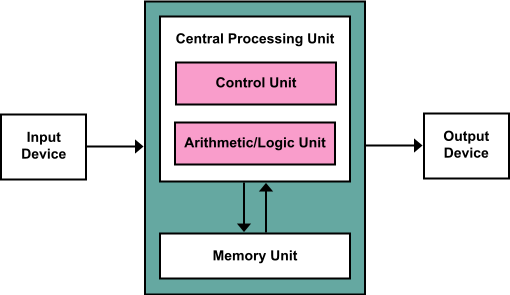
\includegraphics[width=10cm]{Images/Von_Neumann_Architecture.png}
       \caption{Von Neumann architecture.}
           \label{Fig:VonNeumannArch}
\end{figure}

\href{https://commons.wikimedia.org/wiki/File:Von_Neumann_Architecture.svg}{citation for von neumann architecture image}

The von Neumann architecture has several limitations, with one of the biggest criticisms being that it is bottlenecked by the throughput between the CPU and memory.
Essentially, the CPU will eventually have more processing power than the bus can handle to write/read from memory.
This causes the CPU to wait until the bus is freed to continue processing.
As an alternative, we will now look at the Harvard Architecture

The Harvard architecture looks at the problem as says that if the CPU is too large and complex, then each individual component should be separated.
This allows for the tasks to be distributed evenly amongst the several smaller components like the ALU and Instruction memory as opposed to having them live inside the CPU.
The CPU is capable of simultaneous reads and writes.
However, a similar bottleneck occurs where the bus connecting each of the components is the limiting factor.
Below is a diagram demonstrating the Harvard Architecture.

\begin{figure}[htb]
    \centering
    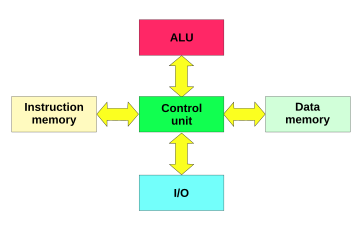
\includegraphics[width=10cm]{Images/Harvard_architecture.svg.png}
       \caption{Harvard architecture.}
           \label{Fig:HarvardArch}
\end{figure}

\href{https://commons.wikimedia.org/wiki/File:Harvard_architecture.svg}{citation for harvard architecture image}

However, modern day computers utilize a mixed computer architecture called the Modified Harvard architecture.
It combines both architectures into a single model.
This usually is of the form of separating the components of the computer, but allowing several smaller memory caches for the CPU.
This is why modern computers utilize several components such as the CPU, GPU, Main Memory (SDD or HDD) and so forth.
Furthermore, this advancement allows for paralellism or multi-core systems to arise.
Some notable examples include the NVIDIA RTX 4080 which has over 8000 cores \href{https://www.techpowerup.com/gpu-specs/geforce-rtx-4080.c3888}{SOURCE} or for the intel i9-13900ks CPU to have 16 cores \href{https://www.intel.com/content/www/us/en/products/sku/232167/intel-core-i913900ks-processor-36m-cache-up-to-6-00-ghz/specifications.html}{SOURCE}.
By allowing each one to independently operate, but still have the CPU as the "brains" of the operation.
We will now dive slightly deeper into the discussion to see what lies beneath these components within modern computer systems.

\subsubsection{Logic Gates}

The basic building blocks for devices such as the ALU, CPU, and such are logic gates.
These are simplistic logical components that allow for processing of data and performing operations on them.

The core of the CPU relies on the ALU.
The ALU is contains registers which simply hold data inside.
Registers are associated with an address for referencing purposes.

Within the ALU there are smallers components that perform specific operations such as addition and subtraction.
These smaller components utilize logical gates such as the OR gate to compute the result with the given input.

\subsection{Constructing the TM}

With the ability to construct logic gates, we can create more complex components such as the ALU, CPU, and more.
Accompanied with the ability to store memory, as well as have a way to interact with the system through Input and Output, we are able to create a functional computer.
In these examples below, these developers have successfully created Computers in Minecraft and Terraria respectively
\href{https://www.youtube.com/watch?v=CW9N6kGbu2I}{Computer in Minecraft}
\href{https://www.youtube.com/watch?v=zXPiqk0-zDY}{Computer in Terraria}.
In fact, we will see later on that the computer built inside Terraria is verifiably TC via a method introduced in \ref{subsubsec:CGoL}

This means that to construct a TM on a physical level (of course assuming unbounded memory), these would be the minimum requirements.

\section{Computer Science}

\subsection{State Machines}

\subsubsection{Formal Technical Writing}

$\lambda \gamma \tau $ etc. being used to describe TC

\subsubsection{Gamified Writing}

$\lambda \gamma \tau $ etc. being used to describe TC, but based on a very verbose and interactive style

\subsection{Software Implementation}

Demonstrate an example of a problem/scenario which shows TC.

\subsubsection{Conway's Game of Life}\label{subsubsec:CGoL}

Classic example to implement

\subsubsection{Rule 110}

Simpler example to implement

\subsubsection{Calculator with Store Value}

More challenging to implement than the previous two.

\subsection{Interpreter for a known Turing Complete language}

Implement an interpreter for a known TC language in a given language.
Must faithfully and accurately simulate the behavior of the given language to be interpreted.

typically, we will implement a simple TC language such as brainfuck

\section{Mathematics}

\subsection{Lambda Calculus}

Basically a simplistic view of math functions.
can be shown as TC through construction of certain concepts.